\documentclass[11pt, a4paper, titlepage]{report}
\linespread{1.2}
\usepackage[polish]{babel}
\usepackage[utf8]{inputenc}
\usepackage{polski}
\usepackage[T1]{fontenc}
\usepackage{graphicx}
\usepackage{enumitem}
\usepackage[hidelinks]{hyperref}
\usepackage{afterpage}
\usepackage{listings}
\usepackage{color}
\frenchspacing
\addtolength{\textwidth}{3.5cm}
\addtolength{\hoffset}{-2cm}
\addtolength{\textheight}{3.5cm}
\addtolength{\voffset}{-2cm}
\usepackage{indentfirst}
\usepackage{caption}
\definecolor{mygreen}{rgb}{0,0.6,0}
\definecolor{mygray}{rgb}{0.5,0.5,0.5}
\definecolor{mymauve}{rgb}{0.58,0,0.82}

\renewcommand\lstlistlistingname{Spis listingów}
\lstset{ %
  language=Matlab,
	backgroundcolor=\color{white},   % choose the background color
	basicstyle=\footnotesize,        % size of fonts used for the code
	breaklines=true,                 % automatic line breaking only at whitespace
	frame=single,
	commentstyle=\color{mygreen},    % comment style
	escapeinside={\%*}{*)},          % if you want to add LaTeX within your code
	keywordstyle=\color{blue},       % keyword style
	stringstyle=\color{mymauve},     % string literal style
}
\date{Wrocław, 06.06.2016}
\makeatletter
\renewcommand{\maketitle}{\begin{titlepage}
		\begin{center}\small
			Politechnika Wrocławska\\
			Wydział Elektroniki\\
			Rok akad. 2015/2016\\
			Kierunek Informatyka\\
			\vspace{3cm}
			\rule{\linewidth}{0.4pt}
				\huge \textsc{\textbf{Komputerowe wspomaganie diagnozowania choroby niedokrwiennej u dzieci z wykorzystaniem algorytmów minimalno-odległościowych}}
				\vspace{0.5cm} \\
				\normalsize \textit{Zastosowanie informatyki w medycynie: Projekt}
			\rule{\linewidth}{0.4pt}
		\end{center}

		\vspace{3cm}
		\begin{flushleft}
			\textbf{\textit{Grupa projektowa:}} \hspace{6.5cm} \textbf{\textit{Prowadzący:}} \\
			Barłomiej Grzegorek, 200814 \hfill{prof. dr hab. inż. Marek Kurzyński} \\
			Marcin Mantke, 200633\\
			\vspace{2cm}
		\end{flushleft}
		\vspace*{\stretch{6}}
		\begin{center}
			\@date
		\end{center}
	\end{titlepage}%
}
\makeatother
\begin{document}
\maketitle
\tableofcontents
\cleardoublepage
\phantomsection
\addcontentsline{toc}{chapter}{\listfigurename}
\listoffigures

\cleardoublepage
\phantomsection
\addcontentsline{toc}{chapter}{Spis listingów}
\lstlistoflistings
\chapter{Charakterystyka analizowanego problemu}
\label{chap:Charakterystyka analizowanego problemu}
Poruszany w niniejszej pracy problem dotyczy wspomagania diagnozowania choroby niedokrwiennej u  dzieci z wykorzystaniem algorytmów minimalno-odległościowych. Główną częścią pracy jest analiza problemu klasyfikacji, na podstawie udostępnionych danych. Najważniejszym zadaniem klasyfikacji jest zbudowanie modelu, który będzie w stanie przypisywać nowe obiekty, do znanych już klas. Do tego celu wykorzystywane są zebrane wcześniej dane, stanowiące tzw. zbiór treningowy.\\

Do badań wykorzystane zostały dane zawierające 410 obiektów o znanych klasach– które w tym przypadku odzwierciedlają rozpoznane rodzaje choroby niedokrwiennej. Wyróżnionych zostało 20 różnych jednostek chorobowych. Każdy z obiektów opisany jest łącznie za pomocą 32 cech, które oznaczają wyniki badań pojedynczego pacjenta. Cechy zostały podzielone na grupy opisujące odpowiednio:
\begin{itemize}
  \item obraz krwi,
  \item obraz szpiku,
  \item stan komórki,
  \item osocze,
  \item test odpornościowy,
  \item test urobylinowy, urobilinogenowy, urobilirubinowy,
  \item test ruchliwości komórki,
  \item wrażenia kliniczne.
\end{itemize}

Podane cechy mają charakter dyskretny oraz są wielowartościowe – w zależności od rodzaju mogą przyjmować od 2(cechy binarne) do 6 różnych wartości.\\
Podczas badań przetestowana została jakość klasyfikacji obiektów w zależności od różnych parametrów budowy klasyfikatora, np. różne rodzaje pomiaru odległości.

\chapter{Opis stosowanych algorytmów}
\label{chap:Opis stosowanych algorytmów}
\section{Metryka odległości}
\label{sec:Metryka odległosci}
W algorytmach odległościowych istotną rolę odgrywa wybrana metryka wg której mierzone będzie odległość pomiędzy dwoma badanymi punktami. Spośród wielu wybrane zostały metryka euklidesowa i metryka Manhattan.
\subsubsection{Metryka euklidesowa}
\label{subs:Metryka euklidesowa}
Metryka euklidesowa, w której za odległość między dwoma punktami w przestrzeni przyjmuje się pierwiastek euklidesowego iloczynu skalarnego różnicy dwóch wektorów:
$$d_e(x,y) = \sqrt{(y-x, x-y)}$$
Przykład:
\begin{figure}[h]
  \centering
  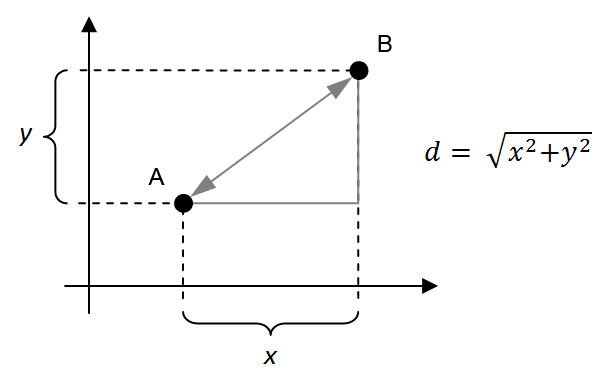
\includegraphics[scale=0.5]{obrazki/euklides}
  \caption{Przykład obliczania metryki eukliesowej.}
\end{figure}
\subsubsection{Metryka Manhattan}
\label{subs:Metryka Manhattan}
Metryka Manhattan, w której odległość dwóch punktów to suma wartości bezwzględnych różnic ich współrzędnych, zgodnie z poniższym wzorem:
$$d_m(x,y) = \sum\limits_{k=1}^n |x_k - y_k|$$
Przykład:
\begin{figure}[h]
  \centering
  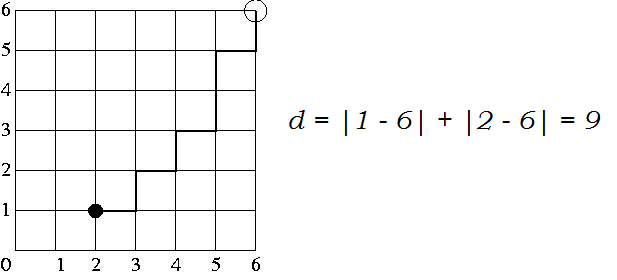
\includegraphics[scale=0.5]{obrazki/manhattan}
  \caption{Przykład obliczania metryki manhattan.}
\end{figure}

\section{Algorytm nearest neighbour}
\label{sec:Algorytm nearest neighbour}
Algorytm k-NN pozwala wyszukać w zadanym zbiorze punktów, k punktów znajdujących się najbliżej nowego punktu, korzystając przy tym z wybranej miary odległości.\\
W zagadnieniu klasyfikacji, algorytm k-NN przyjmuje jako argument tzw. zbiór uczący składający się z wielowymiarowych wektorów cech oraz przypisanych do nich klas. Faza klasyfikacji nowego obiektu polega na przypisaniu odpowiedniej klasy nieznanemu wektorowi cech. Nowy obiekt przypisywany jest do klasy, która występuje najczęściej wśród k najbliżej znajdujących się obiektów ze zbioru uczącego, zgodnie z wybraną metryką. Specjalnym przypadkiem algorytmu jest sytuacja, w której $k = 1$. Nazywa się algorytmem najbliższego sąsiada, w którym klasa nowego obiektu ustalana jest na podstawie najbliżej leżącej próbki ze zbioru danych uczących. Na poniższym rysunku przestawiona została przykładowa przestrzeń zawierająca dane uczące (niebieskie kwadraty oraz czerwona trójkąty) oraz niezidentyfikowaną próbkę – zielone kółko):
\begin{figure}[h]
  \centering
  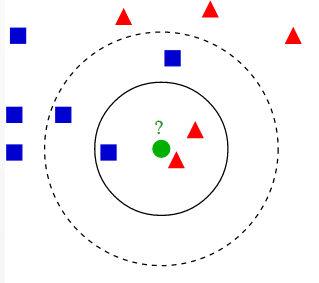
\includegraphics[scale=0.5]{obrazki/knn}
  \caption{Klasyfikacja w algorytmie k-nn.}
\end{figure}

Przyjmując liczbę najbliższych sąsiadów $k = 3$ (ciągła linia na rysunku),  nowy obiekt zostanie przypisany do grupy czerwonych trójkątów, ponieważ jest ich więcej wśród 3 najbliższych próbek. Przyjmując $k = 5$, nowy obiekt zostanie przypisany do klasy niebieskich kwadratów, ponieważ w najbliższym otoczeniu znajdują się 3 kwadraty i tylko 2 trójkąty.

\section{Algorytm nearest mean}
\label{sec:Algorytm nearest mean}
Algorytm nearest mean jest jednym z algorytmów minimalnoodległościowych. Jest on wykorzystywany w statystyce to prognozowania wartości pewnej zmiennej losowej bądź do zadania klasyfikacji.

Założenia:
\begin{itemize}
  \item dany jest zbiór uczący, który zawiera obserwacje. Każda z obserwacji ma przypisany wektor zmiennych objaśniających $X_1...X_n$ oraz wartość zmiennej objaśnianej $Y$,
  \item dana jest obserwacja $C$ z przypisanym wektorem zmiennch objaśniających $X_1...X_n$ dla której chcemy prognozować wartość zmiennej objaśnianej $Y$.
\end{itemize}

Przebieg algorytmu:
\begin{enumerate}
  \item korzystając ze zbioru uczącego oblicz centroid dla każdej wartości zmiennej objaśnianej $Y$,
  \item zaklasyfikuj obserwację $C$ do jednej z klas zmiennej objaśnianej $Y$ poprzez minimalizację odległości pomiędzy wektorem wybranych cech, a centroidem.
\end{enumerate}

\chapter{Implementacja}
\label{chap:Implementacja}
\section{Informacja o środowisku implementacyjnym}
\label{sec:Informacja o środowisku implementacyjnym}
Algorytmy zostały zaimplementowane w środowisku \textbf{MATLAB}. Ranking cech został uzyskany przy pomocy środowiska \textbf{Orange} (\url{http://orange.biolab.si/}). Jest to rozwiązanie open source, które umożliwia wizualizację oraz analizę~danych.
\section{Ranking cech}
\label{sec:Ranking cech}
Korzystając z narzędzia \textbf{Orange} wygenerowaliśmy ranking cech przedstawiony na rysunku \ref{fig:ranking}.
\newpage
\begin{figure}[h]
  \label{fig:ranking}
  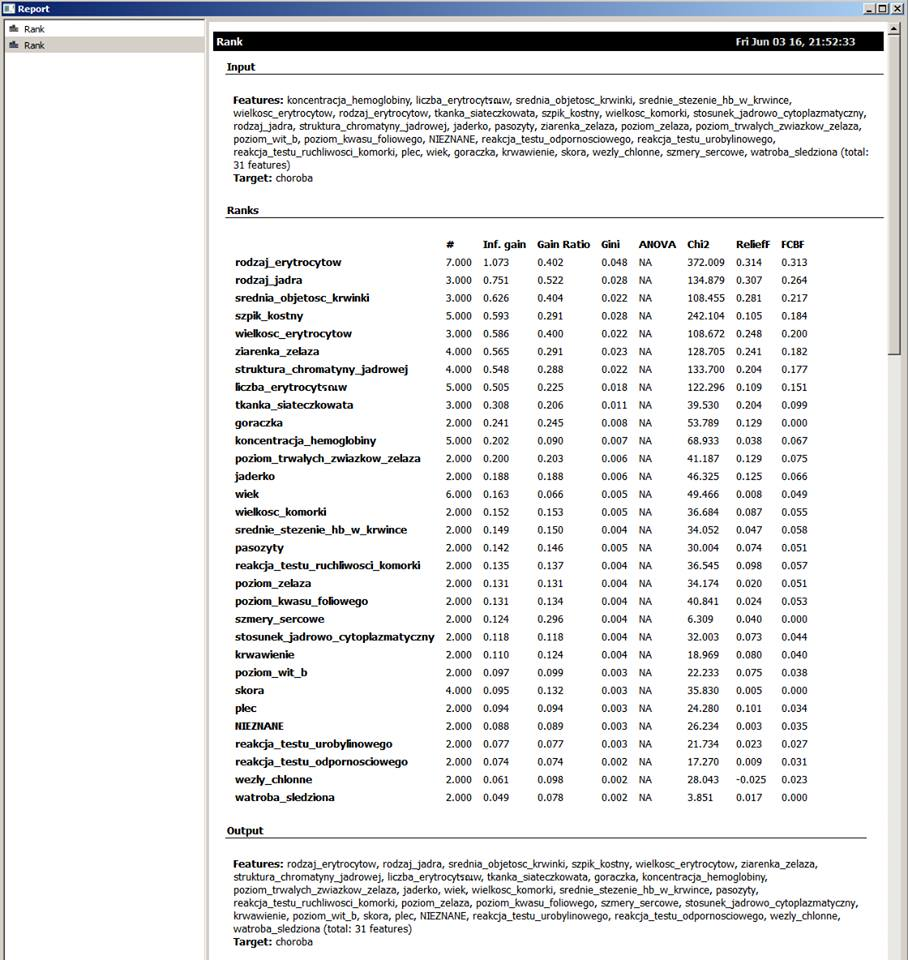
\includegraphics[scale=0.5]{obrazki/ranking}
  \caption{Ranking cech.}
\end{figure}

\section{Implementacja algorytmów}
\label{sec:Implementacja algorytmów}
\subsection{k nearest neighbours}
\label{subs:k nearest neighbours}
Badania eksperymentalne z użyciem algorytmu k najbliższych sąsiadów wykonane zostały – zgodnie z wytycznymi – przy użyciu metody podwójnej walidacji krzyżowej, powtarzanej pięciokrotnie, uśredniając wyniki wszystkich eksperymentów. W tym celu zaimplementowany został algorytm przedstawiony na poniższym listingu:\\

\begin{lstlisting}[label={lst:knn},caption={Algorytm walidacji krzyżowej dla algorytmu kNN.}]
function [ result ] = knn( features, neighbors, standardize, distanceMetric )
  feature_rank = [6, 11, 3, 8, 5, 15, 12, 2, 7, 26, 1,
    17, 13, 25, 9, 4, 14, 23, 16, 19, 30,
    10, 27, 18, 28, 24, 20, 22, 21, 29, 31];
  data = load('dane.txt');
  data = getBestRankedFeatures(data, feature_rank(1:features));

  result = 0;
  N = 5;
  for i = 1 : N
      [train, test] = splitDataRandomly(data);
      Mdl = buildKnnClassifier(train, neighbors,
        standardize, distanceMetric);
      [count, percentage] = getScore(Mdl, test);

      Mdl1 = buildKnnClassifier(test, neighbors,
        standardize, distanceMetric);
      [count1, percentage1] = getScore(Mdl1, train);

      result = result + (percentage + percentage1) / 2;
    end
  result = result / N;
end
\end{lstlisting}

Ranking cech, którego sposób wyznaczenia opisany został w rozdziale \ref{sec:Ranking cech}, przechowywany jest w wektorze \textit{feature\_rank}. Pierwszym krokiem algorytmu jest załadowanie danych wejściowych wraz z przypisanymi do nich klasami oraz wybranie z nich podanej w parametrze liczby najlepszych cech.
Następnie w wykonującej się pięciokrotnie pętli, wyselekcjonowane dane dzielone są losowo na 2 równe podzbiory – uczący(train) oraz testujący(test), na podstawie których budowane są 2 klasyfikatory. Poniżej przedstawiona została implementacja funkcji wykorzystanej do budowy klasyfikatora:\\

\begin{lstlisting}[label={lst:knn_klasyfikator},caption={Budowa klasyfikatora kNN.}]
function [ Mdl ] = buildKnnClassifier( trainData, NumNeighbors, Standardize, Distance)
%BUILDKNNCLASSIFIER Builds knn classifier
    X = trainData(1:end,2:end); % train data without classes
    Y = trainData(1:end,1:1);   % array of training data classes
    Mdl = fitcknn(X, Y, 'NumNeighbors', NumNeighbors, 'Standardize', Standardize, 'Distance', Distance);
end
\end{lstlisting}

Następnie klasyfikator zbudowany na podstawie podzbioru train testowany jest na podzbiorze test, natomiast klasyfikator zbudowany na podstawie zbioru test testowany jest na podzbiorze train. Do celów testowania klasyfikatora wykorzystana została funkcja predict klasy ClassificationKNN, przyporządkowująca podanym danym testowym klasy, na podstawie podanego w parametrze wytrenowanego klasyfikatora. Metoda wykorzystana została w zaimplementowanej funkcji getScore, która jednocześnie zlicza poprawnie zaklasyfikowane obiekty:\\

\begin{lstlisting}[label={lst:knn_test},caption={Testowanie oraz badanie jakości klasyfikatora kNN.}]
function [ count, percentage ] = getScore( classifier, testData )
    T = testData(1:end,2:end);             % test data without class labels
    label = predict(classifier, T);        % predicted classes
    result = [label, testData(:,1)];
    count = 0;
    for i = 1:size(result,1)
        if result(i,1) == result(i,2)
            count = count + 1;
        end
    end
    percentage = count/size(result,1) * 100;
end
\end{lstlisting}
\subsection{Nearest mean}
\label{subs:Nearest mean}
Na poniższych listingach przedstawione są najważniejsze części programów.

\begin{lstlisting}[label={lst:podzial},caption={Podział danych na zbiór uczący i testowy.}]
data = data(randperm(end), :);
train = data(1:floor(0.5*size(data, 1)), :);
test = data(floor(0.5*size(data, 1))+1:end, :);
\end{lstlisting}

\begin{lstlisting}[label={lst:centroidy},caption={Etap treningu - wyznaczanie centroidów.}]
centroid = [unique(data(:, 1)) zeros(size(unique(data(:, 1)), 1), size(data, 2)-1)];

for label = unique(train(:, 1))'
    % zbierz wszystkie próbki danej klasy
    train(train(:, 1) == label, 2:end)
    % oblicz centroid dla danej klasy
    centroid(centroid(:, 1) == label, 2:end) = mean(train(train(:, 1) == label, 2:end));
end
\end{lstlisting}

\begin{lstlisting}[label={lst:pre_result},caption={Wyznaczenie odległości próbki od centroida i przydzielenie do klasy.}]
pre_result = zeros(size(test, 1), 1);
for i = 1:size(test, 1)
    dist = pdist2(test(i, feature_rank(1:k)), centroid(:, feature_rank(1:k)));
    [~, templabel] = min(dist);
    pre_result(i) = centroid(templabel, 1);
end
\end{lstlisting}

\chapter{Opis badań eksperymentalnych}
\label{chap:Opis badań eksperymentalnych}
Badania eksperymentalne zostały przeprowadzone zgodnie z instrukcją. Zastosowano trenowanie i testowanie klasyfikatorów z wykorzystaniem 5 razy powtarzanej metody 2-krotnej walidacji krzyżowej. Zastosowane miary odległości to miara euklidesowa i Manhattan.
\section{Wyniki badań}
\label{chap:Wyniki badań}
\subsection{Algorytm nearest neighbour}
\label{subs:Algorytm nearest neighbour}
\subsubsection{Liczba uwzględnionych cech}
\label{subs:Liczba uwzględnionych cech}
Najniższa jakość klasyfikatora, niezależnie od innych parametrów, osiągana była przy uwzględnianiu najmniejszej liczby cech z rankingu. Wartość dla wszystkich 12 przypadków wywołań algorytmu z uwzględnieniem tylko pierwszej cechy z rankingu wahała się od: 12,68\% (dla neighbors = 1, standardize = true, distanceMetric = Manhattan) do 19,325 (dla neighbors = 13, standardize = false, distanceMetric = Manhattan).
We wszystkich przypadkach najwyższy skok jakościowy został odnotowany po uwzględnieniu kolejnej cechy z rankingu. Dla dwóch najlepszych cech, wyniki wynosiły od 23,66\% (dla neighbors = 1, standardize = false, distanceMetric = Euklidesowa), do 34,44\% (dla neighbors = 13, standardize = false, distanceMetric = Euklidesowa).\\

Rysunek \ref{fig:knn_res} przedstawia wykres zależności ilości branych pod uwagę cech od skuteczności klasyfikacji, dla czterech opisanych wyżej przypadków.
\begin{figure}[h]
  \centering
  \label{fig:knn_res}
  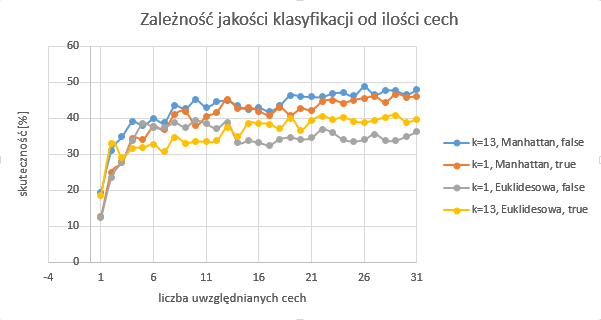
\includegraphics[scale=0.8]{obrazki/knn_plot}
  \caption{Wynik badań dla algorytmu knn.}
\end{figure}
Największy wzrost jakości widoczny jest do momentu dodania 6. cechy. Dodawanie kolejnych cech w niewielkim stopniu zmienia jakoś algorytmu – nie zawsze na lepszą.

\subsubsection{Liczba sąsiadów}
\label{subs:Liczba sąsiadów}
Do testów wybrano 3 różne liczby określające wśród ilu najbliższych sąsiadów należy szukać klasy wzorca: $k=1$, $k=6$ oraz $k=13$.
Wpływ różnej liczby sąsiadów na jakość klasyfikacji uzależniona jest także od zastosowanej metryki. Jak zostało wykazane w badaniach, stosując metrykę Manhattan 72\% wyników zwiększa swoją jakość klasyfikacji, gdy zwiększona zostaje liczba uwzględnianych sąsiadów. Analogicznie, dla metryki Euklidesowej wynik ten wynosi zaledwie 36,3\%.

\subsubsection{Najlepszy wynik}
\label{subs:Najlepszy wynik}
Przeprowadzając badania dla wszystkich 12 przypadków oraz 31 możliwości wyboru liczby cech, najlepsze osiągnięte wyniki wynoszą od 35,37\%  (dla neighbors = 13, standardize = false, distanceMetric = Euklidesowa, uwzględniając 5 najlepszych cech) do 48,05\% dla  (dla neighbors = 13, standardize = true, distanceMetric = Manhattan, uwzględniając 24 cechy).

\subsubsection{Weryfikacja algorytmu}
\label{subs:Weryfikacja algorytmu}
W celu weryfikacji poprawności działania zaimplementowanego algorytmu oraz skryptu testującego, przeprowadzone zostało analogiczne badanie, w którym klasyfikatory testowane były tymi samymi danymi, na których były uczone. Zgodnie z przewidywaniami, jakoś wyników znacznie wzrosła, utrzymując się na poziomie 90\% - 100\% poprawnych wyników dla wszystkich możliwych kombinacji parametrów. Test ten potwierdza poprawność działania samych klasyfikatorów oraz procesu ich uczenia.
\newpage
\subsection{Algorytm nearest mean}
\label{subs:Algorytm nearest mean}
Wyniki badań dla algorytmu nearest mean zostały przedstawione na rysunku \ref{fig:nm_res}.

\begin{figure}[h]
  \centering
  \label{fig:nm_res}
  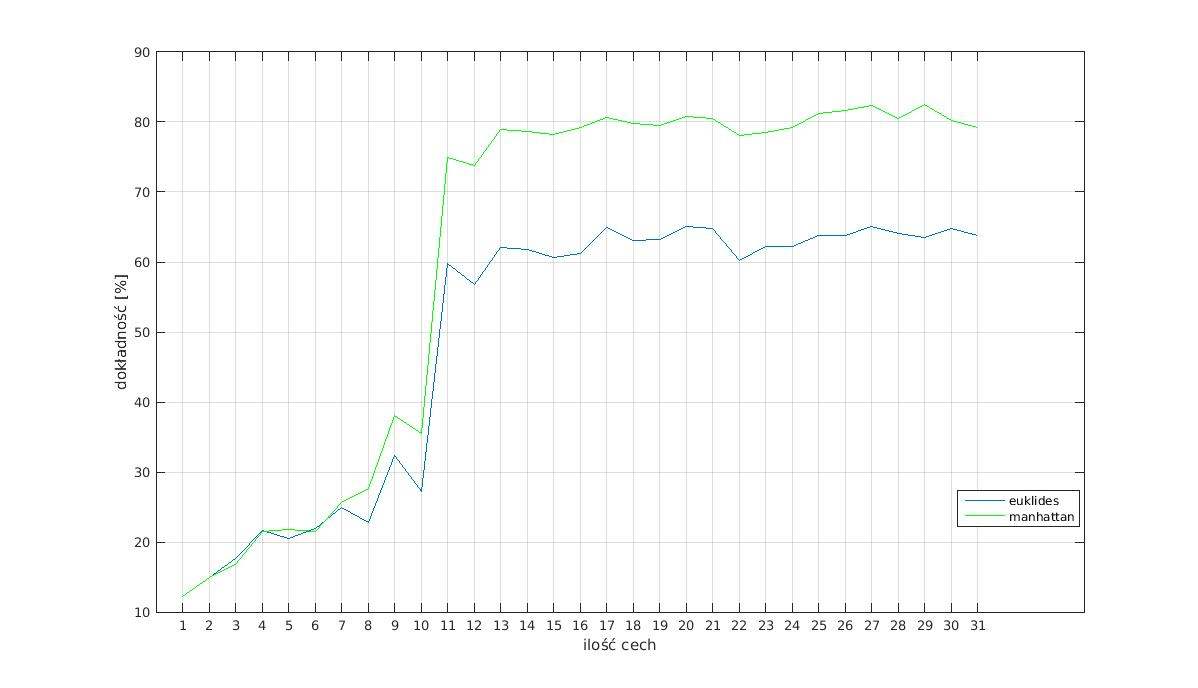
\includegraphics[scale=0.4]{obrazki/nm_plot}
  \caption{Wynik badań dla algorytmu nearest mean.}
\end{figure}

Jak widać na rysunku, dokładność klasyfikacji rośnie wraz ze zwiększaniem liczby cech biorącej udział w klasyfikacji. Największy skok dokładności występuje przy wykorzystaniu 11 cech (różnica na poziomie 40\%). Kolejne zwiększanie ilości cech utrzymuje dokładność klasyfikacji na względnie równym poziomie (nie ma dużych wzrostów ani spadków dokładności klasyfikacji).\\
Z rysunku można również odczytać, że wpływ na dokładność klasyfikacji ma wybrana metryka. Od momentu dołożenia 11 cechy, czyli największego wzrostu dokładności klasyfikacji, klasyfikacja dla metryki euklidesowej jest średnio 25-30\% gorsza od metryki Manhattan.

\chapter{Podsumowanie i wnioski}
\label{chap:Podsumowanie i wnioski}
\section{Wnioski płynące z analizy wyników}
Wspólną cechą obu algorytmów wynikającą z analizy wyników badań jest wyższość metryki Manhattan nad metryką euklidesową. W obu przypadkach metryka ta dawała o wiele lepsze wyniki.
Porównując wyniki badań obu algorytmów można znaleźć sporo różnic. Pierwszą i najważniejszą jest dokładność klasyfikacji. Algorytm kNN był w stanie poprawnie przydzielić jedynie 48\% próbek, natomiast NM ponad 80\%. Te wyniki zostały jednak osiągnięte przy różnych ilościach cech branych pod uwagę w algorytmie - dla kNN były to 24 cechy, natomiast dla NM 17. Różnica występowała również w momencie znacznego zwiększenia dokładności klasyfikacji w zależności do ilości cech. W przypadku kNN skok występował już przy użyciu 6 cech, natomiast algorytm NM zwiększał swoją dokładność od 11 cech, więc prawie dwa razy więcej od kNN. Algorytmy te różniły się również stopniem poprawy dokładności wyników. Dla kNN było to 5-10\%, natomiast dla NM aż 30\%. Biorąc pod uwagę wszystkie z wymienionych powyżej różnic można stwierdzić, że algorytm nearest mean nadaje się lepiej do realizacji zadania wspomagania diagnozowania choroby niedokrwiennej u dzieci.
\section{Ocena krytyczna i podsumowanie projektu}
Realizację projektu można uznać za zadowalającą. W trakcie implementacji spore problemy przysporzyło nam zagadnienie selekcji cech. Niestety nie udało nam się znaleźć odpowiednich materiałów, dzięki którym moglibyśmy zaimplementować selekcję cech przy pomocy kryterium Kołmogorowa. Zamiast tego został wykorzystany dodatkowy program służący do analizy danych, gdzie jest zaimplementowana funkcja generująca ranking cech.

\end{document}
